\documentclass{beamer}

\usepackage{ucs}
\usepackage[utf8x]{inputenc}
\usepackage[T1]{fontenc}
\usepackage[english]{babel}

\usepackage[retainorgcmds]{IEEEtrantools}%	IEEEeqnarray

\usepackage{mathabx}%	convolution symbol
\usepackage{multi row}
\usepackage{epstopdf}
\usepackage{listings}
\lstset{
	language=c,
	basicstyle=\footnotesize,
	showtabs=true,
	tabsize=3,
}

%	presentation info
\title{Roofline and Matrix Multiplication PAPI Analysis}

\author{José Alves, Rui Brito}

\institute[pg22765, pg22781]{
	Universidade do Minho
}

\date{Braga, November 2012}


%	beamer options
\usetheme{Frankfurt}


\begin{document}%	begin presentation

\maketitle%	title slide

\begin{frame}
	\frametitle{Index}
	\tableofcontents
\end{frame}

\begin{frame}
	\frametitle{Sources for Machine Specifications}

	Sources used for a complete profile:
	\begin{description}
		\item[Linux System Information] (/proc/cpuinfo, /proc/meminfo) To gather specifications on hardware;\\
		\item[Web] (ark.intel.com, crucial.com) For micro architecture and memory specifications;\\
		\item[Linux Tools and Packages] (dmidecode, sysctl, bandwidth) To gather memory, cpu and bandwidth info;\\
	\end{description}

\end{frame}
\section{Specifications}
\begin{frame}
	\frametitle{Machines Specs}
	{\small
	\begin{table}[!htp]
		\begin{tabular}{lrl}
			\hline 
			\textbf{Manufacter:} & Apple \\
			\hline \\
			\textbf{Model:} & MacBook Pro late 2008 \\
			\hline 
			\textbf{Processor} & & \\
			Manufacturer: & Intel & \\
			Arch: & Core & \\
			Model: & Core 2 Duo T9600 & \\
			Cores: & 2 & \\
			Clock Frequency: & 2.80 GHz & \\
			FP Performance's Peak: & 44.8 GFlops/s & \\
			\hline
			\end{tabular}
		\caption{MacBook Pro late 2008 specifications}
		\label{tab:mbp}
\end{table}
}
\end{frame}
\begin{frame}
	\frametitle{Machines Specs}
	{\small
	\begin{table}[!htp]
		\begin{tabular}{lrl}
			\hline 
			\textbf{Cache} & & \\
			Level: & 1 & \\
			Size: & 32KB + 32KB & \\
			Line Size: & 64 B & \\
			Associative: & 8-way & \\
			Memory Access Bandwidth: & 40 GB/s & \\
			\\
			Level: & 2 & \\
			Size: & 6 MB & \\
			Line Size: & 64 B & \\
			Associative: & 24-way & \\
			\hline 
			\textbf{RAM} \\
			Type: & SDRAM DDR3 PC3-8500 & \\
			Frequency: & 1067 MHz & \\
			Size: & 4 GB & \\
			Num. Channels: & 2 & \\
			Latency: & 13.13 ns & \\
		\end{tabular}
		\caption{MacBook Pro late 2008 specifications}
		\label{tab:mbp}
\end{table}
}
\end{frame}
\begin{frame}
	\frametitle{Machines Specs}
	{\small
	\begin{table}[!htp]
		\begin{tabular}{lrl}
			\hline 
			\textbf{Manufacter:} & HP \\
			\hline 
			\textbf{Model:} & Pavillion dv6-2190ep \\
			\hline 
			\textbf{Processor} & & \\
			Manufacturer: & Intel & \\
			Arch: & Nehalem & \\
			Model: & i7-720QM & \\
			Cores: & 4 & \\
			Clock Frequency: & 1.60 GHz & \\
			FP Performance's Peak: & 51.2 GFlops/s & \\
			\hline 
			\end{tabular}
		\caption{HP Pavillion dv6-2190ep specifications}
		\label{tab:mbp}
\end{table}
}
\end{frame}
			\begin{frame}
	\frametitle{Machines Specs}
	{\small
	\begin{table}[!htp]
		\begin{tabular}{lrl}
		\hline
			\textbf{Cache} & & \\
			Level: & 1 & \\
			Size: & 32KB + 32KB & \\
			Line Size: & 64 B & \\
			Associative: & 4/8-way & \\
			Memory Access Bandwidth: & 22 GB/s & \\
			\\
			Level: & 2 & \\
			Size: & 256 KB & \\
			Line Size: & 64 B & \\
			Associative: & 8-way & \\
			\\
			Level: & 3 & \\
			Size: & 6 MB & \\
			Line Size: & 64 B & \\
			Associative: & 12-way & \\
			\hline 
			\textbf{RAM} \\
			Type: & SDRAM DDR3 PC3-10600 & \\
			Frequency: & 1333 MHz & \\
			Size: & 4GB & \\
			Num. Channels: & 2 & \\
			Latency: & 13.5 ns & \\
		\end{tabular}
		\caption{HP Pavillion dv6-2190ep specifications}
		\label{tab:mbp}
\end{table}
}
\end{frame}



\section{Roofline}
\begin{frame}
	\begin{figure}[!htp]
		%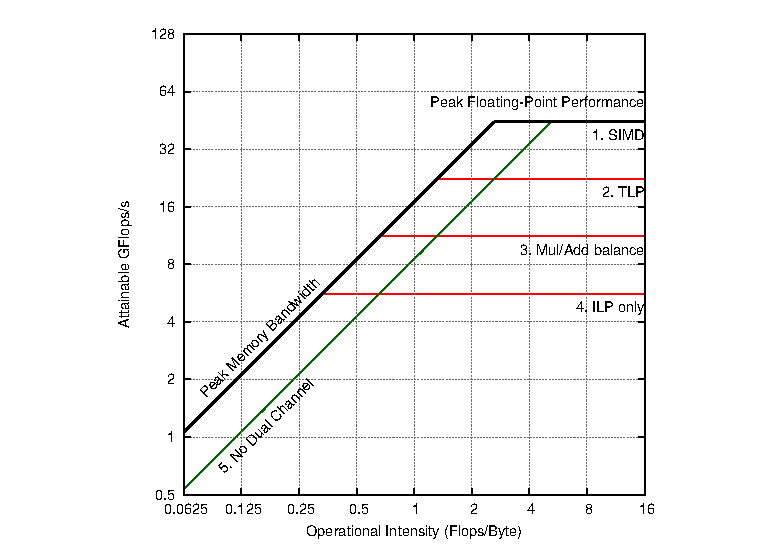
\includegraphics[width=12cm]{images/roofline.eps}
		\label{fig:roofline}
		\end{figure}
\end{frame}

\section{PAPI Case Study: Matrix Multiplication}
\begin{frame}%	begin slide
	\frametitle{Problem}

	Analyse the performance of a \textbf{matrix multiplication} algorithm, \begin{equation}Matrix A * Matrix B = Matrix C\end{equation} wich contains a triple nested loop with the indexes i,j and k (line,column and position).\\

	The implementation used runs two versions of the problem, one multipying matrixA with matrixB, and another multipying matrixA with the transpose of matrixB.
\end{frame}%	end slide

\begin{frame}[fragile]
	\frametitle{Algorithm}

Standard implementation of a matrix multiplication in C.

\begin{verbatim}
for (i = 0; i < size; i++) {
    for (j = 0; j < size; j++) {
        for(k = 0; k < size; k++) {
            acc += matrixA[i][k] * matrixB[k][j];				
            }		
            matrixC[i][j] = acc;	
            acc = 0;
        }
    }
\end{verbatim}
\end{frame}

\begin{frame}
	\frametitle{Counters Used}

	Used counters gathered by PAPI:
	\begin{description}
		\item[PAPI\_TOT\_CYC] Total cycles;
		\item[PAPI\_TOT\_INS] Total instructions
		\item[PAPI\_LD\_INS] Load Instructions
		\item[PAPI\_SR\_INS] Store Instructions
		\item[PAPI\_FML\_INS] Multiply instructions
		\item[PAPI\_FDV\_INS] Division instructions
		\item[PAPI\_VEC\_INS] Vector Instructions
		\item[PAPI\_FP\_OPS] Floating point operations
		\item[PAPI\_L1\_DCA] L1 data cache accesses
		\item[PAPI\_L1\_DCM] L1 data cache misses
		\item[PAPI\_L2\_DCA] L2 data cache accesses
		\item[PAPI\_L2\_DCM] L2 data cache misses
	\end{description}
\end{frame}

\section{Test cases}
\begin{frame}
	\frametitle{Test cases}

	Test cases were selected to fit on the multiple memory levels.\\
	Each Test case was run 4 times for each version of the problem.

	\begin{center}
		\begin{table}[!htp]
	\begin{tabular}{lrlrlrl}
		\hline
		\textbf{Memory} & \textbf{Size} & \textbf{Matrix Size} \\
		\hline
		L1 & 30 KB & 50 \\
		L2 & 255 KB & 146 \\
		L3 & 3 MB & 500 \\
		RAM & 7.68 MB & 800 \\
		\hline
	\end{tabular}
	\caption{Test cases}
	\label{tab:testcases}
\end{table}
	\end{center}
\end{frame}

\section{Results}
\subsection{Memory Accesses}

\begin{frame}[fragile]
	\frametitle{Memory Accesses: Estimated Value}

	Code structure (based on Assembly analysis):
	\\
	\begin{center}
		\begin{lstlisting}
			for(1 to N) {
			   [4 stores, 1 load, 7 instr.]
			   for(1 to N) {
			      [6 stores, 3 loads, 34 instr.]
			   }
			   [3 stores, 6 loads, 26 instr.]
			}
			for(1 to N) {
			   [3 stores, 3 loads, 10 instr.]
			}
		\end{lstlisting}
	\end{center}
\end{frame}

\begin{frame}
	\frametitle{Memory Accesses: Formula}

	Based on the previous code structure, the number of memory accesses can be estimated with:
	$$9N^{2} + 20N$$
	where N is the number of objects being processed.
	\\
	The total estimated number of instruction is given by:
	$$34N^{2} + 43N$$
\end{frame}

\begin{frame}
	\frametitle{Memory Accesses}

	The following table shows the number of memory accesses, by PAPI readings and by estimation from the previous formula

	\begin{table}[!htp]
		\begin{center}
		{\small
			\begin{tabular}{|l|r|r|c|c|}

				\hline
				Test	&	PAPI					&	Estimated					&	Est. Error			&	 Accesses/Inst		\\
				\hline
				L1\_1	&	38716					&	38144						&	1.50\%				&	0.27						\\
				L1\_2	&	150588					&	150016						&	0.38\%				&	0.27						\\
				L2\_1	&	604144268				&	604143616					&	0.00\%				&	0.26						\\
				L2\_2	&	2416247656				&	2416246784					&	0.00\%				&	0.26						\\
				RAM\_1	&	38656024690				&	38656016384					&	0.00\%				&	0.26						\\
				RAM\_2	&	154621476174			&	154621444096				&	0.00\%				&	0.26						\\
				\hline
			\end{tabular}
		}
		\end{center}
	\end{table}
\end{frame}

\subsection{Mul/Add balance}
\begin{frame}
	\frametitle{Mult/Add balance}

	There is no counter for Add operations, so it was estimated with
	$$PAPI\_FP\_INS - PAPI\_FML\_INS - PAPI\_FDV\_IN$$

	\begin{table}[!htp]
		\begin{center}
		{\small
			\begin{tabular}{|l|r|r|c|c|}

				\hline
				Test	&	FP Mul Inst		&	FP Add Inst		&	Mul/Add balance	\\
				\hline
				L1\_1	&	33555			&	30395			&	90.58\%			\\
				L1\_2	&	133168			&	117874			&	88.52\%			\\
				L2\_1	&	537008683		&	469949801		&	87.51\%			\\
				L2\_2	&	2147782971		&	1879409199		&	87.50\%			\\
				RAM\_1	&	34360620752		&	30066293472		&	87.50\%			\\
				RAM\_2	&	137440660580	&	120261583165	&	87.50\%			\\
				\hline
			\end{tabular}
		}
		\end{center}
	\end{table}
\end{frame}

\subsection{CPI}
\begin{frame}
	\frametitle{CPI}

	Calculated based on FPI\_TOT\_INS and FPI\_TOT\_CYC

	\begin{table}[!htp]
		\begin{center}
		{\small
			\begin{tabular}{|l|r|r|c|c|}

				\hline
				Test	&	Instructions	&	Cycles			&	CPI		&	IPC		\\
				\hline
				L1\_1	&	143317			&	135750			&	0.95	&	1.06	\\
				L1\_2	&	563861			&	472027			&	0.84	&	1.19	\\
				L2\_1	&	2282055015		&	1686732377		&	0.74	&	1.35	\\
				L2\_2	&	9127511619		&	6775496328		&	0.74	&	1.35	\\
				RAM\_1	&	146031715237	&	171062387955	&	1.17	&	0.85	\\
				RAM\_2	&	584121221418	&	687083107943	&	1.18	&	0.85	\\
				\hline
			\end{tabular}
		}
		\end{center}
	\end{table}
\end{frame}

\subsection{Miss rates}
\begin{frame}
	\frametitle{Miss rates}% %miss / case size

	Based on the counters that give total accesses and misses to both L1 and L2 cache levels

	\begin{table}[!htp]
		\begin{center}
		{\small
			\begin{tabular}{|l|r|r|c|c|}

				\hline
				Test	&	L1 Accesses		&	L1 Miss \%	&	L2 Accesses		&	L2 Miss \%	\\
				\hline
				L1\_1	&	50287			&	0.20\%		&	290				&	33.79\%		\\
				L1\_2	&	194416			&	0.10\%		&	476				&	34.03\%		\\
				L2\_1	&	750943668		&	11.18\%		&	219910694		&	0.01\%		\\
				L2\_2	&	3007631681		&	11.18\%		&	882123490		&	0.01\%		\\
				RAM\_1	&	48304577585		&	11.14\%		&	10917610760		&	46.85\%		\\
				RAM\_2	&	194497858380	&	11.06\%		&	42817380648		&	50.25\%		\\
				\hline
			\end{tabular}
		}
		\end{center}
	\end{table}
\end{frame}

\subsection{Operational Intensity}
\begin{frame}
	\frametitle{Operational Intensity}

	Attempted to estimate Bytes read from RAM with L2\_MISSES * 64, assuming that every miss will issue a new cache line read from RAM (64 Bytes)
	However:
	\begin{itemize}
		\item L2 counters are derived (maybe not reliable?)
		\item \#L1 misses <> \#L2 accesses. So we can also assume that \#L2 misses <> \#RAM accesses, making the previous formula wrong
	\end{itemize}

	\begin{table}[!htp]
		\begin{center}
		{\small
			\begin{tabular}{|l|r|r|r|r|}
				\hline
				Test	&	L2 Misses		&	Bytes from RAM		&	FP Inst.		&	Op. Intensity	\\
				\hline
				L1\_1	&	98				&	6272				&	68110			&	10.86			\\
				L1\_2	&	162				&	10368				&	267551			&	25.81			\\
				L2\_1	&	11434			&	731776				&	1074075321		&	1,467.77		\\
				L2\_2	&	103001			&	6592064				&	4295643580		&	651.64			\\
				RAM\_1	&	5114423222		&	0.3e+11 (0.3 TB)	&	68721939721		&	0.21			\\
				RAM\_2	&	21517065599		&	1.3e+12 (1.3 TB)	&	274882221251	&	0.20			\\
				\hline
			\end{tabular}
		}
		\end{center}
	\end{table}

	Actually, 1.3 TB is near the calculated value that should be read from RAM if there was no cache in between.\\
	$$N^{2} \times 80 Bytes = 131072^{2} \times 80 Bytes = 1.25 TB$$

	So given the 50\% Miss Rate from L2 Cache, it was expected that the number of Bytes read from RAM was around half, or 0.65 TB, which is not the case.\\

		For L2 Tests, the very high Operational Intensity is due to an increase of the data set (L2\_1 is 64 times bigger than L1\_2) but still with enough size to fit in L2 cache, which lowers the number of reads from RAM.

\end{frame}

\section{Conclusion}
\begin{frame}
	\frametitle{Conclusion}
	\begin{itemize}
		\item Some difficulties measuring memory ceilings. The Roofline paper used a custom Stream benchmark, and provided no theorethical way to estimate those values;
		\item PAPI counters may sometimes differ from what is expected, especially when measuring memory traffic;
		\item TLP was not explored, and it would certainly prove beneficial and easili implemented for this particular algorithm;
	\end{itemize}
\end{frame}

\section{Questions}
\begin{frame}
	\titlepage
	
	
\end{frame}

\end{document}%	end presentation